
NFAC and Cacla are going to be compared in two continuous environments : Acrobot and Cartpole.
Acrobot (double swing-up) is an under actuated arm of two-link. The first joint
cannot exert torque where the second can.
It always begin in the same position (straight down).
The reward function is defined as 1) +1 if the goal is reached, 2) normalized max 
height of end effector if 500 step are reached, 3) 0 otherwise.

Cartpole or inverted pendulum is also made of 2 joints. The first joint is a pivot point 
between the cart and the pole, where torques cannot be applied. The other joint controls
the horizontal movement of the cart.
The reward function is defined as +1 everywhere.

\begin{figure*}[h]
\centering
\begin{minipage}{.5\textwidth}
  \centering
  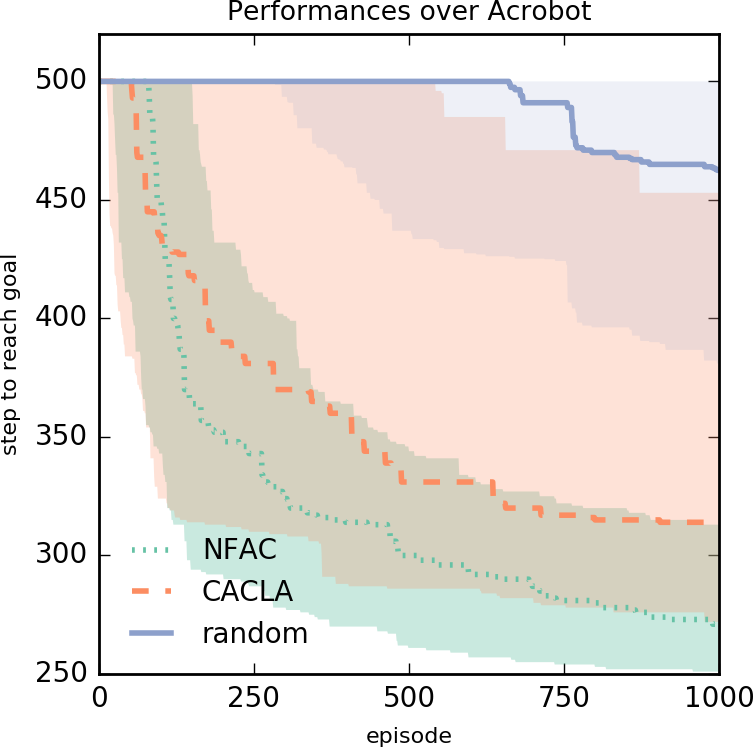
\includegraphics[width=0.95\linewidth]{result_plotting/adacrobot-1ddl_perf.png}
\end{minipage}%
\begin{minipage}{.5\textwidth}
  \centering
  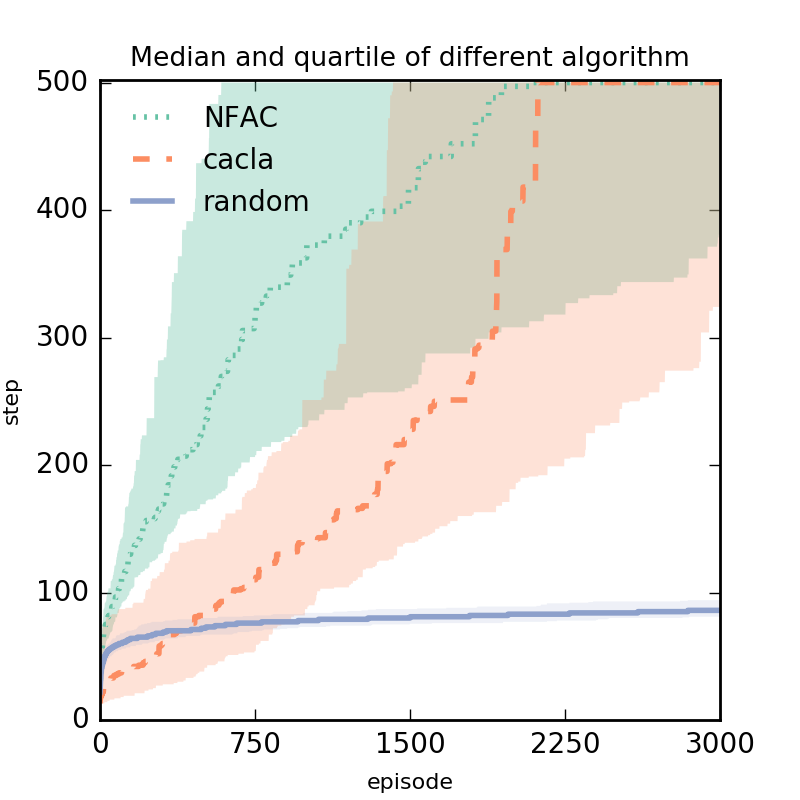
\includegraphics[width=0.95\linewidth]{result_plotting/cartpole_perf.png}
\end{minipage}
\caption{ \label{fig:actions} Median and quartile of performance in Acrobot (lower better) and Cartpole (higher better) environment during RL learning.}
\end{figure*}


In acrobot, 75\% of NFAC agents reach their goal after only 151 episodes where cacla agents need 544 episodes. The median shows that the quality
of the policies found by NFAC are better. After 1000 episodes, 75 \% of NFAC agents can reach the goal after only 313 steps versus 453 steps for cacla.

In cartpole, 25\% of NFAC agents can preserve the goal during 500 steps after 623 episodes versus 1419 episodes for cacla. The median of NFAC is better 
than cacla during the first episodes then converge after 2200 episodes.

Statistics have been made over 150 different runs after meta-parameters optimization for each algorithms
(the number of hidden units for the policy is the same).
For acrobot $\epsilon$-greedy policies are used, instead with cartpole gaussian policies are used.